\documentclass[a4paper]{article}

%use the english line for english reports
%usepackage[english]{babel}
\usepackage[portuguese]{babel}
\usepackage[utf8]{inputenc}
\usepackage{indentfirst}
\usepackage{graphicx}
\usepackage{verbatim}


\begin{document}

\setlength{\textwidth}{16cm}
\setlength{\textheight}{22cm}

\title{\Huge\textbf{Breakthru}\linebreak\linebreak\linebreak
\Large\textbf{Relatório Final}\linebreak\linebreak
\linebreak\linebreak

\includegraphics[scale=0.1]{feup-logo.png}\linebreak\linebreak
\linebreak\linebreak
\Large{Mestrado Integrado em Engenharia Informática e Computação} \linebreak\linebreak
\Large{Programação em Lógica}\linebreak
}

\author{\textbf{Grupo Breakthru 2:}\\
João Rafael de Figueiredo Cabral - 201304395 \\
João Bernardo Martins de Sousa e Silva Mota - 201303462 \\
\linebreak\linebreak \\
 \\ Faculdade de Engenharia da Universidade do Porto \\ Rua Roberto Frias, s\/n, 4200-465 Porto, Portugal \linebreak\linebreak\linebreak
\linebreak\linebreak\vspace{1cm}}

\maketitle
\thispagestyle{empty}

\section{Resumo}
No contexto da unidade curricular Programação em Lógica do MIEIC foi solicitada a implementação de um jogo de tabuleiro a ser selecionado pelo grupo.

Para a implementação deste jogo o grupo mobilizou os seus conhecimentos acerca de PROLOG e das capacidades generativas que o mesmo proporciona e que se revelaram de elevada importância para permitir o desenvolvimento de um jogo do ponto de vista declarativo, tornando-se apenas necessário explicitar em PROLOG as regras de funcionamento do jogo.

O acima exposto evidencia a acentuada diferença paradigmática da programação nesta linguagem, que representou para o grupo um desafio mas também uma oportunidade de adquirir destreza mental no que à programação em lógica diz respeito.



\tableofcontents
\newpage

\section{Introdução}
Foi proposta a implementação do jogo \textit{Breakthru} em PROLOG com uma interface textual e com a possibilidade de ser jogado em três modos diversos: humano contra humano, humano contra máquina e máquina contra máquina. Foi solicitado que o mecanismo de jogo da máquina apresentasse dois níveis distintos de dificuldade.

O presente relatório principia por apresentar o jogo desenvolvido, o seu contexto histórico e as regras que o regem. De seguida são apresentadas as principais estruturações programáticas do mesmo, do ponto de vista do modelo de dados usado e dos predicados lógicos fundamentais da implementação desenvolvida. Em particular é apresentada a representação interna do estado do jogo, os predicados usados para apresentar externamente essa mesma representação, bem como diversos predicados e restante lógica de movimentação de peças que permita verificar o cumprimento das regras por parte dos jogadores humanos e a escolha de jogadas por parte do computador, quando em controlo de um dos jogadores. São depois tecidas considerações sobre a interface com o utilizador e suas funcionalidades e implementação.

Encerra-se o relatório com uma breve reflexão sobre o trabalho desenvolvido, suas limitações e aspetos que ficam em aberto para eventuais futuras melhorias.

\section{O Jogo Breakthru}
O \emph{Breakthru} é um jogo de estratégia abstrata para dois jogadores em que cada lado começa com um número diferente de peças, colocadas em posições assimétricas e com objetivos diferentes para assegurar a vitória.

\subsection{História}
O jogo foi criado em 1965 por Alex Randolph, com um conjunto de regras baseadas nas do \emph{Hnefatafl}\footnote{https://boardgamegeek.com/boardgame/335/breakthru}, um jogo de estratégia abstrata cuja popularidade remonta à Escandinávia medieval, existindo vestígios da sua presença entre várias civilizações antigas\footnote{https://boardgamegeek.com/boardgame/2932/hnefatafl}.
\

\subsection{Regras}
\subsubsection{Peças}
A cor de cada jogador é sorteada através do lançamento de uma moeda, sendo que o jogador vencedor desse sorteio é o jogador dourado e o perdedor é o jogador prateado. O tabuleiro conta com 13 peças douradas, das quais 12 dispostas em quadrado à volta da 13ª peça, no centro do tabuleiro, e de 20 peças prateadas dispostas em volta das peças douradas.

O jogador dourado dispõe as suas 12 peças normais como desejar na zona central do tabuleiro, nele delimitada. O jogador prateado procede de forma semelhante, dispondo contudo as suas 20 peças fora da zona central, reservada ao jogador dourado.

Uma das peças douradas é diferente das restantes, sendo designada por navio almirante. A sua posição inicial é fixa, sendo obrigatório que seja colocada no centro do tabuleiro.

\subsubsection{Movimentos e Capturas}
Cada jogador deve, na sua vez, efetuar dois movimentos ou uma captura. O jogador dourado escolhe quem deve jogar primeiro.

Todas as peças podem ser movimentadas um número arbitrário de espaços livres na horizontal ou vertical, à semelhança do movimento de uma torre no xadrez. Durante o movimento nenhuma peça pode saltar por cima de outra ou ocupar uma casa já ocupada, como ilustrado na figura \ref{fig:moves}.

As capturas são feitas movimentando uma peça para uma casa que lhe seja diagonalmente adjacente e que esteja ocupada por uma peça do adversário, como ilustrado na figura \ref{fig:captures}, sendo esta removida do jogo.

Quando o navio almirante dourado efetua um movimento o jogador dourado não pode efetuar outro movimento nesse turno.

\subsubsection{Objetivo do Jogo}
O jogador prateado ganha o jogo ao capturar o navio almirante dourado. O jogador dourado ganha o jogo se o navio almirante chegar a uma das casas exteriores do tabuleiro.

\begin{figure}
\centering
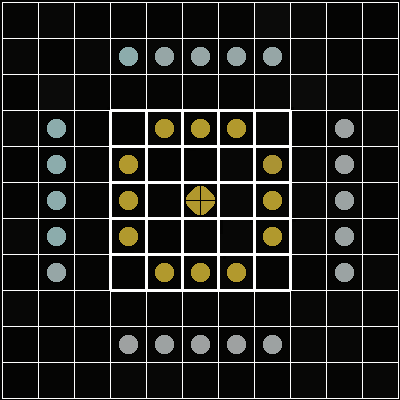
\includegraphics[scale=1]{Breakthru_board.png}
\centering
\caption{Uma posição inicial possível das peças num tabuleiro de Breakthru}
\label{fig:init}
\end{figure}
\begin{figure}
\centering
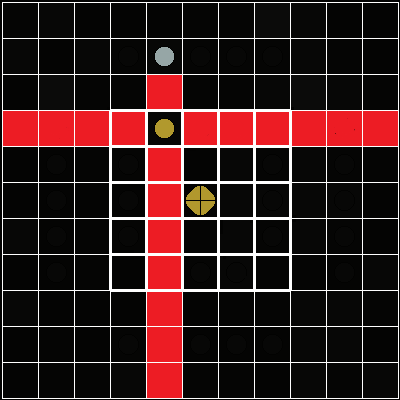
\includegraphics[scale=1]{Breakthru_moves.png}
\caption{A vermelho: movimentos possíveis da peça dourada}
\label{fig:captures}
\end{figure}

\begin{figure}
\centering
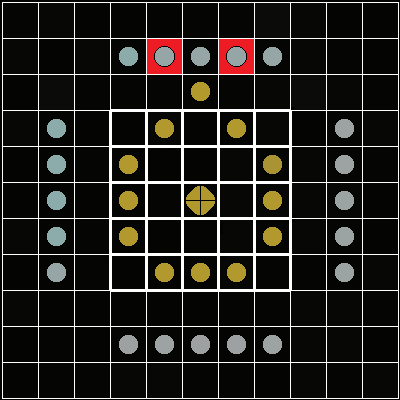
\includegraphics[scale=1]{Breakthru_capture.png}
\caption{A vermelho: capturas possíveis da peça dourada}
\label{fig:moves}
\end{figure}

\section{Lógica do Jogo}
Será exposta ao longo desta secção do relatório a forma como são implementados os diversos aspetos que tornam o Breakthru jogável.

%%%%%%%%%%%%%%%%%%%%%%%%%%
\subsection{Representação do Estado do Jogo}
O tabuleiro está definido através de chamadas ao predicado \textit{position}. Cada célula do tabuleiro unifica com o átomo \textit{emptyCell}, podendo ainda as células que alojam peças unificar com as mesmas. Um exemplo de utilização deste predicado seria:
\textit{position(5, 5, flagship).}

%%%%%%%%%%%%%%%%%%%%%%%%%%
\subsection{Visualização do Tabuleiro}

Foram desenvolvidos alguns predicados em PROLOG para permitir a visualização do tabuleiro usando caracteres \textit{ASCII}, como exemplificado pela figura \ref{fig:example}.
\begin{figure}
\centering
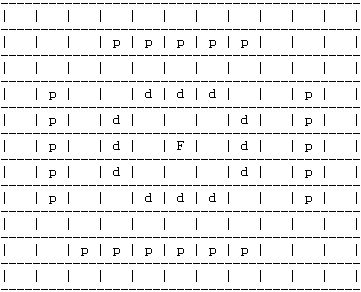
\includegraphics[scale=1]{Breakthru_initial_sicstus.png}
\caption{Tabuleiro inicial de um jogo de Breakthru}
\label{fig:example}
\end{figure}

\subsubsection{Predicados de Visualização}
Foram implementados os predicados de visualização que se seguem:

\begin{verbatim}
printBoard:- clearScreen, printBoard(0,0),!.

printBoard(_,11):- write(' ----------------------------------------------'),nl,
	write('   0   1   2   3   4   5   6   7   8   9  10'), nl.
printBoard(X,Y):- Y1 is Y+1,
 write(' ---------------------------------------------'),nl,
 write(Y),
 printBoardLine(X,Y),
 printBoard(X,Y1).

printBoardLine(11,_):- write('|'), nl.
printBoardLine(X,Y):- X1 is X+1, position(X,Y, Piece), symbol(Piece, Symb),
write('|'),write(' '), write(Symb), write(' '), printBoardLine(X1, Y).
\end{verbatim}

%%%%%%%%%%%%%%%%%%%%%%%%%%
\subsection{Lista de Jogadas Possíveis}
De forma a poder gerar jogadas a ser executadas pelo computador, bem como efetuar a validação das jogadas feitas pelos jogadores humanos, desenvolveram-se os seguintes predicados:

\begin{verbatim}
validPlay(X,Y,Xf,Yf,Player):- (validMove(X,Y,Xf,Yf,Player);
validCapture(X,Y,Xf,Yf,Player)),\+moved(X,Y).

validCapture(X,Y,Xf,Yf,Player):- %movimento de captura
 owner(Player, Piece),
 position(X,Y,Piece),
 opponent(Player, Opponent),
 owner(Opponent,OpponentPiece),
 position(Xf,Yf,OpponentPiece),
 (X =:= Xf-1; X =:= Xf+1),
 (Y =:= Yf-1; Y =:= Yf+1).

validMove(X,Y,Xf,Yf, Player):- %movimento normal
owner(Player, Piece),
position(X,Y,Piece),
position(Xf,Yf, emptyCell),
findall(Z, position(Xf,Yf,Z), [emptyCell]),
emptySpace(X,Y,Xf,Yf).
\end{verbatim}

Nestes predicados, começa-se por verificar a presença de uma peça pertencente ao jogador que efetua o turno nas coordenadas de início. De seguida, no caso de um movimento normal, verifica-se se das coordenadas de início até às coordenadas de destino existe um caminho aberto, ou seja, se não há peças nas células que existem entre estas. Por outro lado, no caso de um movimento de captura, verifica-se a existência de uma peça pertencente ao oponente nas coordenadas de destino, e vê-se se o movimento é diagonal e de apenas um espaço.

\subsection{Execução de jogadas}
Para a execução de jogadas, foram implementados diversos predicados que lidam com o facto de as jogadas poderem vir a ser feitas por um jogador humano, bem como geradas pelo computador. São eles:

\begin{verbatim}
doPlay(X,Y,Xf,Yf,Player):- validMove(X,Y,Xf,Yf,Player),
	owner(Player,Piece),retract(position(X,Y,Piece)),
	asserta(position(Xf,Yf,Piece)), asserta(moved(Xf,Yf)).

doPlay(X,Y,Xf,Yf,Player):- validCapture(X,Y,Xf,Yf,Player),
	owner(Player,Piece), retract(position(X,Y,Piece)),
	opponent(Player, Opponent), owner(Opponent,OpponentPiece),
	retract(position(Xf,Yf,OpponentPiece)), asserta(position(Xf,Yf,Piece)),
	asserta(captured),
	asserta(moved(Xf,Yf)).

\end{verbatim}

No \textit{Breakthru}, uma jogada pode ser composta pelo movimento de duas peças diferentes, por uma captura, ou, no caso do jogador dourado, pelo movimento do \textit{flagship}. Assim, sendo os predicados acima mostrados são integrados em predicados que se encarregam de simular o modelo comportamental aqui descritos. Estes predicados são os seguintes:

\begin{verbatim}
takeTurn(goldenPlayer, silverPlayer):-
    playerGolden(human), doPlayerMovement(goldenPlayer), printBoard,
    ( (\+moved(flagship), \+captured, printBoard, doPlayerMovement(goldenPlayer));
    (moved(flagship);captured)),!.

takeTurn(goldenPlayer, silverPlayer):-
    playerGolden(bot), difficulty(goldenPlayer, random), randomPlay(goldenPlayer, Pred1),
    Pred =.. Pred1, Pred, printBoard,
    ((\+moved(flagship),\+captured, randomMove(goldenPlayer, Pred2),
    PredD =.. Pred2, PredD);((moved(flagship);captured), printBoard)), !.

takeTurn(goldenPlayer, silverPlayer):-
	 playerGolden(bot), difficulty(goldenPlayer, greedy),
	 ((flagshipCanEscape(Xf, Yf), position(X, Y, flagship),
	 doPlay(X, Y, Xf, Yf, goldenPlayer));
	 (validCapture(X,Y,Xf,Yf, goldenPlayer), doPlay(X,Y,Xf,Yf, goldenPlayer));
	 (randomMove(goldenPlayer, Pred1), Pred =.. Pred1, Pred)),!,
	 (  (moved(flagship);captured;wonGame(_));
	 	 (\+captured,\+moved(flagship),\+wonGame(_), randomMove(goldenPlayer, Pred2),
	 	 PredD =.. Pred2, PredD)),!.


takeTurn(silverPlayer, goldenPlayer):-
    playerSilver(human), doPlayerMovement(silverPlayer), printBoard,
    ((\+captured,doPlayerMovement(silverPlayer));captured),!.

takeTurn(silverPlayer, goldenPlayer):-
    playerSilver(bot), difficulty(silverPlayer, random), randomPlay(silverPlayer, Pred1),
    Pred =.. Pred1, Pred, (captured;(\+captured,randomMove(silverPlayer, Pred2),
    PredD =.. Pred2, PredD)), printBoard, !.

takeTurn(silverPlayer, goldenPlayer):-playerSilver(bot), difficulty(silverPlayer, greedy),
    ( ( blockFlagship(X,Y,Xf,Yf), doPlay(X,Y,Xf,Yf,silverPlayer));
	(validCapture(X,Y,Xf,Yf, silverPlayer), doPlay(X,Y,Xf,Yf,silverPlayer));
	(randomMove(silverPlayer, Pred1), Pred =.. Pred1, Pred)),!,
    (  captured;
	 (\+captured, blockFlagship(X,Y,Xf,Yf), doPlay(X,Y,Xf,Yf,silverPlayer));
	 (\+captured, randomMove(silverPlayer, Pred2), PredD =.. Pred2, PredD)),!.
\end{verbatim}

Estes predicados representam assim o orgão principal de fluxo do jogo, fazendo a gestão de turnos e avançando o jogo através do predicado \textit{doPlay}, que é chamado, no caso em que os jogadores são humanos, no predicado \textit{doPlayerMovement}, que não é aqui exposto por ser um predicado predominantemente de interface com o utilizador. No caso dos jogadores de inteligência artificial, o predicado de execução de jogadas está presente aqui:\\

\textit{randomMove(silverPlayer, Pred1), Pred =.. Pred1, Pred)}\\

Em que Pred será o predicado doPlay.

\subsection{Final do Jogo}

No \textit{Breakthru}, o jogo termina ou quando o \textit{flagship} se encontra numa das células de fora do tabuleiro, ou quando o jogador dourado consegue capturar o \textit{flagship}. Assim, os predicados que verificam o término do jogo esão da seguinte forma:

\begin{verbatim}
wonGame(goldenPlayer):- position(_,0,flagship);position(0,_,flagship);
position(10,_,flagship);position(_,10,flagship);\+position(_,_,silverPiece).
wonGame(silverPlayer):- \+position(_,_,flagship).
\end{verbatim}

Estes predicados são integrados diretamente no ciclo de jogo principal, de forma a que a cada turno se possa efetuar esta verificação:

\begin{verbatim}
 playGame:-
	( (\+playerGolden(bot),readPlayer(Player, 'goldenPlayer chooses a player to start the game
	(goldenPlayer. or silverPlayer.).'));
	(playerGolden(bot), random(0, 2, N), nth0(N, [goldenPlayer, silverPlayer], Player)
	)),
assert(currentPlayer(Player)),
	repeat,
	retract(currentPlayer(CurrentPlayer)),
	retractall(moved(_)), retractall(moved(_,_)),retractall(captured),
	takeTurn(CurrentPlayer, NewPlayer),
	assert(currentPlayer(NewPlayer)),
	printBoard,
	wonGame(Victor),!, clearScreen,
	write(Victor),write(' won the game!').
\end{verbatim}

\subsection{Jogadas do Computador}
Os dois níveis de dificuldade considerados para o computador neste traablho foram, em primeiro lugar, jogadas aleatórias, e em segundo, jogadas de uma natureza gananciosa. Neste último caso, se o computador representar o jogador prateado, a primeira prioridade do mesmo será bloquear o caminho do \textit{flagship} para uma das células de fora, se o mesmo existir. Se não existir este caminho, ou se o jogador prateado não estiver em posição de o bloquear, este efetua uma qualquer captura que esteja disponível. Finalmente, não havendo capturas disponíveis, o computador efetua um movimento aleatório.
Por outro lado, se o computador representar o jogador dourado e se se verificar que existe um caminho aberto entre o \textit{flagship} e uma das células de final, será efetuado o movimento que leva o mesmo até essa célula. Caso contrário o comportamento será análogo ao do jogador dourado (captura ou efetua uma jogada aleatória). Este comportamento está evidenciado em alguns predicados surgidos já na secção 4.4, os quais se mostram também abaixo, por uma questão de praticalidade:

\begin{verbatim}
takeTurn(goldenPlayer, silverPlayer):-
    playerGolden(human), doPlayerMovement(goldenPlayer), printBoard,
    ( (\+moved(flagship), \+captured, printBoard, doPlayerMovement(goldenPlayer));
    (moved(flagship);captured)),!.

takeTurn(goldenPlayer, silverPlayer):-
    playerGolden(bot), difficulty(goldenPlayer, random), randomPlay(goldenPlayer, Pred1),
    Pred =.. Pred1, Pred, printBoard,
    ((\+moved(flagship),\+captured, randomMove(goldenPlayer, Pred2),
    PredD =.. Pred2, PredD);((moved(flagship);captured), printBoard)), !.

takeTurn(goldenPlayer, silverPlayer):-
	 playerGolden(bot), difficulty(goldenPlayer, greedy),
	 ((flagshipCanEscape(Xf, Yf), position(X, Y, flagship),
	 doPlay(X, Y, Xf, Yf, goldenPlayer));
	 (validCapture(X,Y,Xf,Yf, goldenPlayer), doPlay(X,Y,Xf,Yf, goldenPlayer));
	 (randomMove(goldenPlayer, Pred1), Pred =.. Pred1, Pred)),!,
	 (  (moved(flagship);captured;wonGame(_));
	 	 (\+captured,\+moved(flagship),\+wonGame(_), randomMove(goldenPlayer, Pred2),
	 	 PredD =.. Pred2, PredD)),!.


takeTurn(silverPlayer, goldenPlayer):-
    playerSilver(human), doPlayerMovement(silverPlayer), printBoard,
    ((\+captured,doPlayerMovement(silverPlayer));captured),!.

takeTurn(silverPlayer, goldenPlayer):-
    playerSilver(bot), difficulty(silverPlayer, random), randomPlay(silverPlayer, Pred1),
    Pred =.. Pred1, Pred, (captured;(\+captured,randomMove(silverPlayer, Pred2),
    PredD =.. Pred2, PredD)), printBoard, !.

takeTurn(silverPlayer, goldenPlayer):-playerSilver(bot), difficulty(silverPlayer, greedy),
    ( ( blockFlagship(X,Y,Xf,Yf), doPlay(X,Y,Xf,Yf,silverPlayer));
	(validCapture(X,Y,Xf,Yf, silverPlayer), doPlay(X,Y,Xf,Yf,silverPlayer));
	(randomMove(silverPlayer, Pred1), Pred =.. Pred1, Pred)),!,
    (  captured;
	 (\+captured, blockFlagship(X,Y,Xf,Yf), doPlay(X,Y,Xf,Yf,silverPlayer));
	 (\+captured, randomMove(silverPlayer, Pred2), PredD =.. Pred2, PredD)),!.
\end{verbatim}

As jogadas aleatórias são geradas recorrendo às capacidades generativas do PROLOG no predicado \textit{randomPlay} e \textit{randomMove} mostrados abaixo:

\begin{verbatim}
randomMove(CurrPlayer, Pred):-
findall([Xi,Yi,Xf,Yf], validMove(Xi,Yi,Xf,Yf,CurrPlayer), Possiveis),
length(Possiveis, N),
random(0, N, NList),
nth0(NList, Possiveis, ChosenPlay),
append(ChosenPlay, [CurrPlayer], AlmostPred),
append([doPlay], AlmostPred, Pred).

randomPlay(CurrPlayer, Pred):-
findall([Xi,Yi,Xf,Yf], validPlay(Xi,Yi,Xf,Yf,CurrPlayer), Possiveis),
length(Possiveis, N),
random(0, N, NList),
nth0(NList, Possiveis, ChosenPlay),
append(ChosenPlay, [CurrPlayer], AlmostPred),
append([doPlay], AlmostPred, Pred).
\end{verbatim}

No trabalho desenvolvido existe também uma secção do jogo onde os jogadores têm que dispor as peças no tabuleiro da forma que acharem melhor. Também aí se verifica alguma heurística por parte dos jogadores simulados por computador. As peças serão dispostas aleatóreamente por um jogador em modo aleatório, ou, se se tratar do jogador prateado em modo ganacioso, este bloqueará todos os caminhos abertos entre o \textit{flagship} e uma célula de final. Isto é evidenciado nos predicados seguintes:

\begin{verbatim}
randomPlacement(CurrPlayer, X,Y):-
	findall([Xp, Yp], possiblePlace(CurrPlayer, Xp, Yp), Possiveis),
	length(Possiveis, N),
	random(0, N, NList),
	nth0(NList, Possiveis, [X,Y]).

blockFlagship(X,Y,Xj,Yj):-
		position(Xf,Yf,flagship),
		flagshipCanEscape(Xe,Ye),
		((Xe = Xf, Ye > Yf, validMove(X,Y,Xe, Yj,silverPlayer), Yj > Yf, Xj is Xe );
		(Xe = Xf, Ye < Yf, validMove(X,Y,Xe, Yj,silverPlayer), Yj < Yf, Xj is Xe );
		(Ye = Yf, Xe > Xf, validMove(X,Y,Xj, Ye,silverPlayer), Xj > Xf, Yj is Ye );
		(Ye = Yf, Xe < Xf, validMove(X,Y,Xj, Ye,silverPlayer), Xj < Xf, Yj is Ye )).

placePiece(goldenPlayer, 12):- placePiece(silverPlayer, 0).
placePiece(goldenPlayer, N):-playerGolden(human),
	N1 is N+1, N < 12,
	write('New piece for golden player:'), nl,
	repeat,
	readCoordinates(X,Y),
	validateCoordinates(X,Y, goldenPlayer),!,
	asserta(position(X,Y,goldenPiece)),
	printBoard,!,
	placePiece(goldenPlayer, N1).

placePiece(goldenPlayer,N):-
	playerGolden(bot),
	N1 is N+1, N < 12,
	randomPlacement(goldenPlayer, X, Y),
	asserta(position(X,Y,goldenPiece)),
	printBoard,!,
	placePiece(goldenPlayer, N1).

	placePiece(silverPlayer,N):-playerSilver(bot), difficulty(silverPlayer, greedy),
	blockFlagshipPlacement, N1 is N-1, printBoard, !, placePiece(silverPlayer, N-1).

	placePiece(silverPlayer,N):-
		playerSilver(bot),
		N1 is N+1, N < 20,
		randomPlacement(silverPlayer, X, Y),
		asserta(position(X,Y,silverPiece)),
		printBoard,!,
		placePiece(silverPlayer, N1).


placePiece(silverPlayer, 20).
placePiece(silverPlayer, N):- N1 is N+1, N< 20,
	write('New piece for silver player:'), nl,
	repeat,
	readCoordinates(X,Y),
	validateCoordinates(X,Y, silverPlayer),!,
	asserta(position(X,Y,silverPiece)),
	printBoard,!,
	placePiece(silverPlayer, N1).


possiblePlace(Player, X, Y):-
	position(X,Y,emptyCell),
	findall(C, position(X,Y,C), [emptyCell]),
	validateCoordinates(X,Y,Player)
\end{verbatim}


\section{Interface com o utilizador}
Para o presente trabalho foi implementada, para comunicação com um utilizador humano uma interface textual em linha de comandos. Esta interface é constituída maioritariamente por menus iniciais, onde o jogador pode configurar o modo em que quer jogar (humano contra humano, etc...), bem como a dificuldade a dos jogadores simulados por computador e ainda, no caso do modo \textit{humano contra computador}, o utilizador que o jogador humano deseja representar (jogador dourado ou jogador prateado).
Além das interfaces, existem ainda predicados que ao utilizador escrever na consola as coordenadas das peças a mover, bem como as coordenadas de destino das mesmas.

\begin{verbatim}
getInt(X, Value):- repeat,
			write('Value for '), write(Value), write(': '),
			read(X1),
			integer(X1),
			X is X1,
			!.

readCoordinates(X1, Y1):-
 getInt(X1, 'x'),nl,
 getInt(Y1, 'y').

readPlayer(X, Prompt):-
	repeat,
	write(Prompt), nl,
	read(X),
	player(X),!.


mainMenu:-
write('Welcome to Breakthru!'), nl, nl,
write('What would you like to do: '), nl,
write('1. Play game'), nl,
write('2. Tutorial'), nl,
write('3. Exit'), nl,
repeat,
getInt(Option, 'option'),
(Option = 1, clearScreen, playMenu;
Option = 2, clearScreen, tutorial;
Option = 3).

playMenu:-
write('How would you like to play: '), nl,
write('1. Player vs Player'), nl,
write('2. Player vs Bot'), nl,
write('3. Bot vs Bot'), nl,
repeat,
getInt(Option, 'option'),
(Option = 1, clearScreen, assert(playerGolden(human)),
assert(playerSilver(human)), startGame;
Option = 2, clearScreen, chooseSideMenu, startGame;
Option = 3, clearScreen, assert(playerGolden(bot)), botDiffMenu(goldenPlayer),
assert(playerSilver(bot)), botDiffMenu(silverPlayer), startGame).

botDiffMenu(Player):-
	write('Choose bot difficulty for '), write(Player), write(': '), nl,
	write('1. Random Mode'), nl,
	write('2. Greedy Mode'), nl,
	repeat,
	getInt(Option, 'option'),
	(Option = 1, clearScreen, assert(difficulty(Player, random));
	Option = 2, clearScreen, assert(difficulty(Player, greedy))).

chooseSideMenu:-
	readPlayer(Player, 'Choose which side you want to be on (silverPlayer. or goldenPlayer.)'),
	(Player = goldenPlayer, assert(playerGolden(human)),
	assert(playerSilver(bot)), botDiffMenu(silverPlayer);
	Player = silverPlayer, assert(playerSilver(human)),
	assert(playerGolden(bot)), botDiffMenu(goldenPlayer)).
\end{verbatim}

\section{Conclusão}
Ficaram, no entender do grupo, fortemente evidenciadas as vantagens situacionais do uso do paradigma em causa para abordar a classe de problemas que frequentemente surgem no desenvolvimento de simuladores de jogos de tabuleiros. Com efeito, o trabalho desenvolvido evidencia que, recorrendo a capacidades que são exclusivas da programação em lógica, se torna possível exprimir de forma sucinta funcionalidades de um programa que se revelariam de elevada complexidade, do ponto de vista da implementação. O PROLOG permite em larga medida que o programador prescinda da necessidade de especificar um modelo de execução, o que constitui, regra geral, o maior desafio para a implementação deste tipo de programas.

O trabalho apresenta como principal limitação o facto de a inteligência artificial implementada para o segundo nível de dificuldade não apresentar uma função de avaliação do tabuleiro plenamente desenvolvida. A lógica de avaliação implementada é essencialmente binária: a máquina procura a cada passo garantir somente que não vai perder no passo seguinte e que captura ao adversário o máximo de peças possíveis, sendo que os restantes movimentos são selecionados, à falta de heurística desenvolvida, de uma forma aleatória. Considerou-se o desenvolvimento de tal função de avaliação e do seu uso num algoritmo \textit{Minimax}, mas limitações ao nível do tempo e da compreensão plena deste algoritmo, que não foi extensivamente abordado nas aulas da Unidade Curricular, não no-lo permitiram.


\end{document}
